\begin{figure*}[t]
  \centering
  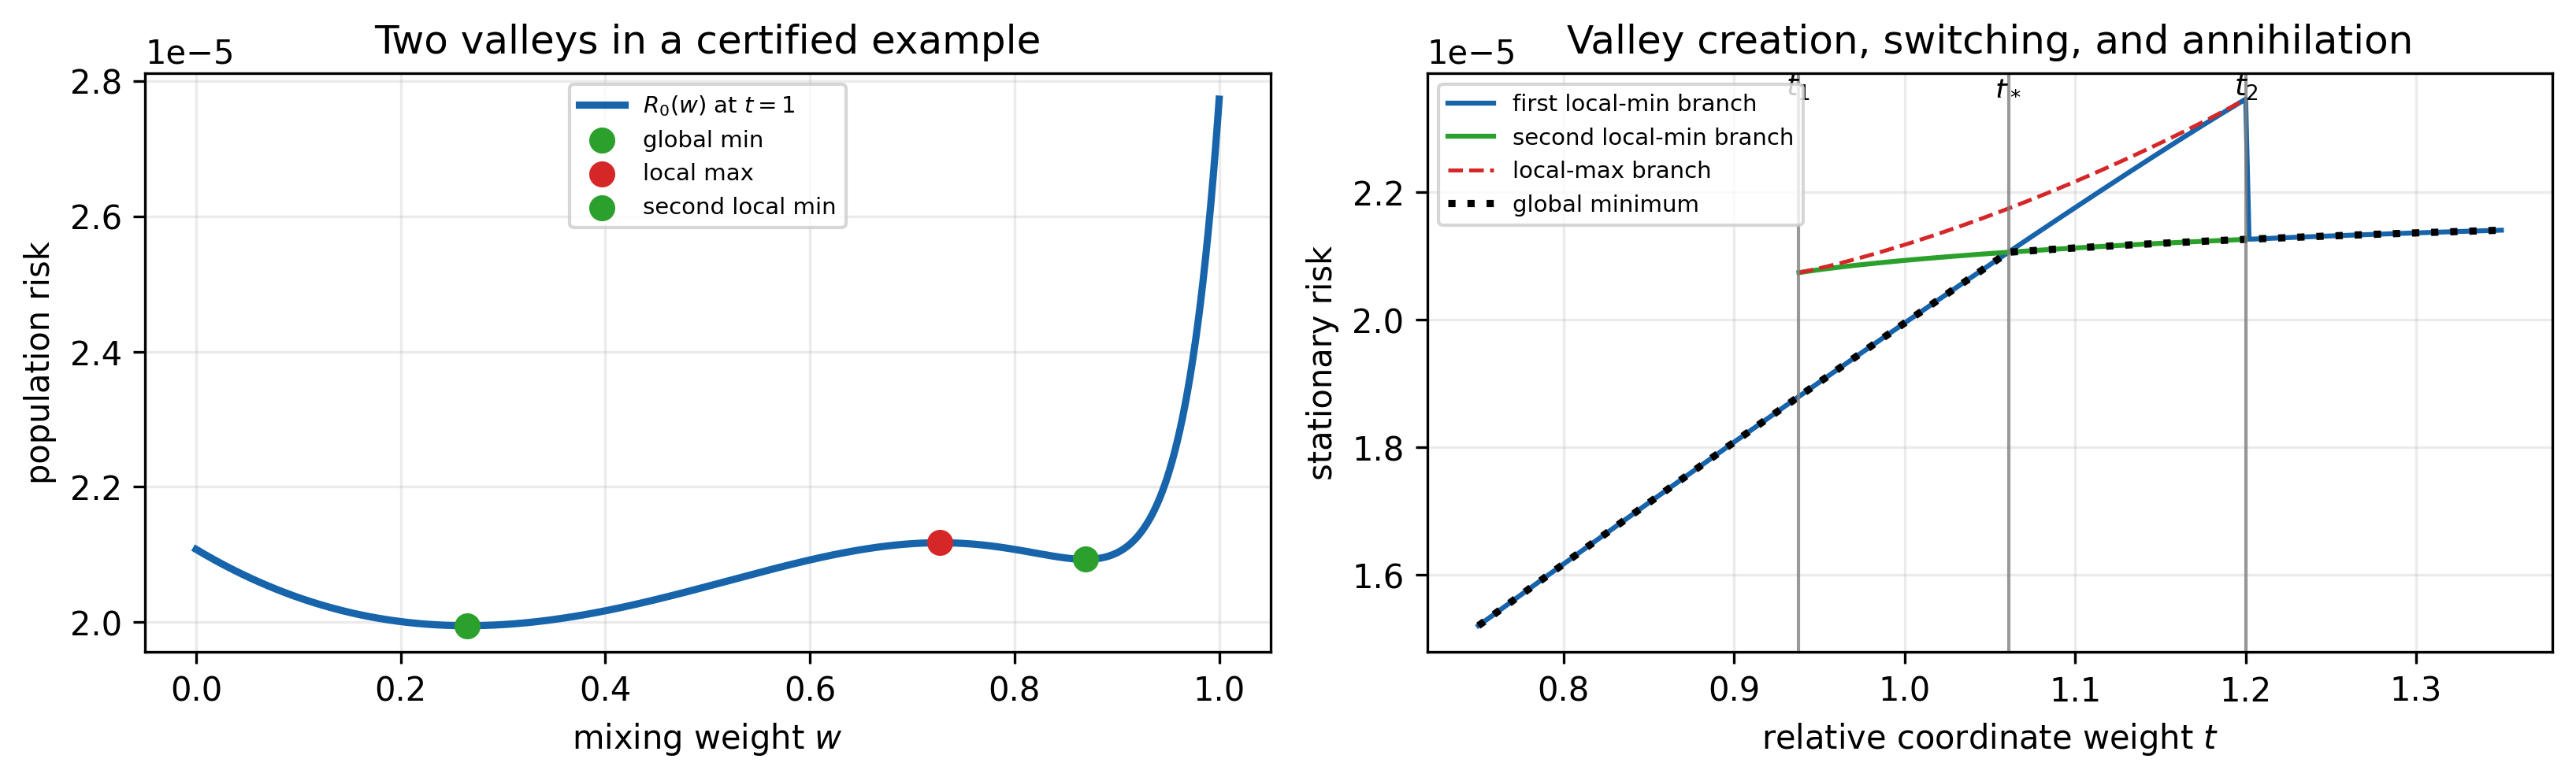
\includegraphics[width=\linewidth]{fig/global_risk_shapes.png}
  \caption{\textbf{Global shapes of auxiliary-data mixing risk.} Left: a certified two-dimensional population risk with two local minima and one local maximum; the first minimum is the unique global optimum. Right: stationary branches of a one-parameter family. Valley pairs appear and disappear at $t_1,t_2$, and at $t_*$ two distinct weights share the global minimum. These are exact algebraic and interval-certified structures, not grid-based shape conjectures.}
  \label{fig:teaser}
\end{figure*}
